\documentclass{amsart}
\usepackage{amsmath}
\usepackage{amssymb}
\usepackage{verbatim}
\usepackage{graphicx}
\usepackage{subfigure}
\usepackage{multicol}
\usepackage{algorithmic}
\usepackage{moreverb}
\usepackage{listings}
\begin{document}

\bigskip
\bigskip
\center{\bf Siarhei Siniak}
\bigskip
\bigskip
\center{\large \bf NMF: Organ phrase analysis}
\center{\large 2016}

\begin{titlepage}

\end{titlepage}

\begin{figure}
  \centering
  \subfigure[Score]{
    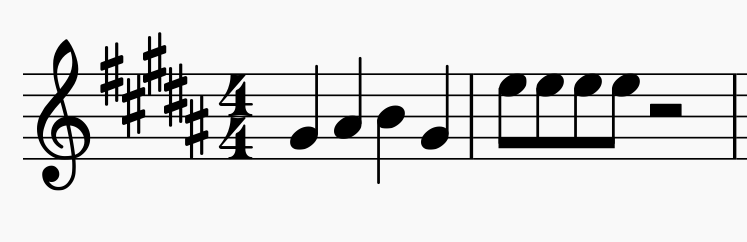
\includegraphics[scale=.5]{res/organ-score.png}}
  \centering
  \caption{Part 1}
    \label{F:5-3-p0}
\end{figure}

\begin{figure}
  \centering
  \subfigure[Spectrogram]{
    \includegraphics[scale=.5]{build/plot_grayscale_spectrogram.png}}\qquad
  \subfigure[Peaks approximation]{
    \includegraphics[scale=.5]{build/test_peaks_detector.png}}\\
  \centering
  \caption{Part 2}
    \label{F:5-3-p1}
\end{figure}

\begin{figure}
  \centering
  \subfigure[Matrix W, frequency profiles]{
    \includegraphics[scale=.5]{build/plot_w_matrix.png}}\qquad
  \subfigure[Matrix H, time parameters]{
    \includegraphics[scale=.5]{build/plot_h_matrix.png}}
  \centering
  \caption{Part 3}
    \label{F:5-3-p2}
\end{figure}

In this here example, we are trying to apply NMF to a real audio sound.
A short organ phrase was taken for a such analysis \cite{L:organ.wav}.
The length of it is 13 seconds. The picture \ref{F:5-3-p0}
presents its score for the first 6 seconds.

You can see the spectrogram on the picture \ref{F:5-3-p1}.
The following were choosen for the analysis.
\begin{verbatim}
  FS = info.SampleRate;
  MFH = 6000;
  M = 2048;
  HS = floor(M * 0.25);
  N = 4096;
  MFS = floor(MFH / FS * N);

  TL = 0.0;
  TR = 5.5;
  SL = floor(TL * FS) + 1;
  SR = floor(TR * FS) + 1;

  x = mean(audioread(info.Filename), 2)(SL : SR);
  [y, c] = stft(x, M, HS, N / 2);
  L = size(y, 2);

  sy = y(1 : MFS, :);

  test_peaks_detector(sy, N, FS);

  plot_grayscale_spectrogram(sy);
\end{verbatim}

The preceeding analysis in Sonic Visualizer \cite{L:sonic-visualizer}
revealed, that it's enough to consider only below 6kHz for frequency domain.

In the appendix D you may see the whole source code in Octave language.

On the following pictures \ref{F:5-3-p2}
are presented results of the NMF algorithm,
i.e. matrices W and H.
The following parameters of NMF were chosen.
\begin{verbatim}
  R = 4;

  [W, H] = innernmf(abs(sy), R, 1e-2);

  plot_h_matrix(L, M, HS, FS, TL, R, H);
  plot_w_matrix(FS, N, MFS, R, W);
\end{verbatim}

To obtain better results, here is a hypothesis:
\begin{enumerate}
  \item Define local peaks on the spectrogram;
  \item Perform their parabollic approximation;
  \item Select stable peaks as frequency funciton of time,
    applying thresholding constraints for deviation;
  \item The resulting form of spectrogram should applied as an input to NMF.
\end{enumerate}

On the picture \ref{F:5-3-p2} you may observe an approximation example.
The very parabollic approximation was applied.

There are a lot of peaks of the low magnitude. Some kind of thresholding
should be applied to get rid of them. It implies input reduction of the NMF
algorithm. That might result in better efficiency.

To improve onset detection NMF should be combined with some other algorithms.

\begin{thebibliography}{0}

  \bibitem{L:organ.wav} https://www.freesound.org/people/nartes/sounds/368365/ 

  \bibitem{L:sonic-visualizer} http://www.sonicvisualiser.org/
\end{thebibliography}

\appendix

\section{D}\label{A:realaudio_nmf_post.m}
\listinginput[1]{1}{src/realaudio_nmf_post.m}

\end{document}
